\chapter{Results}
To evaluate GoSeek's performance, the following tests were conducted. with the documents of size 2000, 10000, and 100000. \\
All of the findings below are condacted on an input of 2 \textbf{.json} files of size up to 300MB - accounting for 100000 html documents after parsing
\begin{itemize}
    \item Search terms - "artificial intelligence","historical figure","climate change"
    \item Patterns searched - "has lost", "given by" , "nowhere else", "warmer than today"
\end{itemize}
\section{Performance}
\subsection{Hardware}
The hardware utilized for the testing phase of this thesis was a laptop equipped with the following specifications:

\begin{itemize}
    \item \textbf{Processor}: AMD Ryzen 7 3750H quad-core processor operating at a base clock speed of 2.3 GHz.
    \item \textbf{Memory}: 8GB of DDR4 RAM.
    \item \textbf{Storage}: A dual-storage configuration comprising a 256GB NVMe SSD for primary operations and a 1TB 5400 rpm HDD for additional storage needs.
    \item \textbf{Graphics}: NVIDIA GeForce GTX 1650 dedicated graphics card, facilitating graphics-intensive operations.
    \item \textbf{Connectivity}: Wi-Fi 5, Bluetooth 4.2, and essential I/O ports, including USB Type-A ports, HDMI, and a combo audio jack.
    \item \textbf{Operating System}: Windows 10 Pro.
\end{itemize}
\subsection{Parsing}
As mentioned in Chapter 2 GoSeek is dependent on 'parse' command to work properly. Figure \ref{fig:cmd-parse} shows the number of seconds it takes GoSeek to parse \textbf{.html} documents into \textbf{.json} for the search and pattern matching functionality While 
figure \ref{fig:memory-usage} shows the memory usage of GoSeek while parsing the docuements.

\begin{figure}[h!]
    \centering
    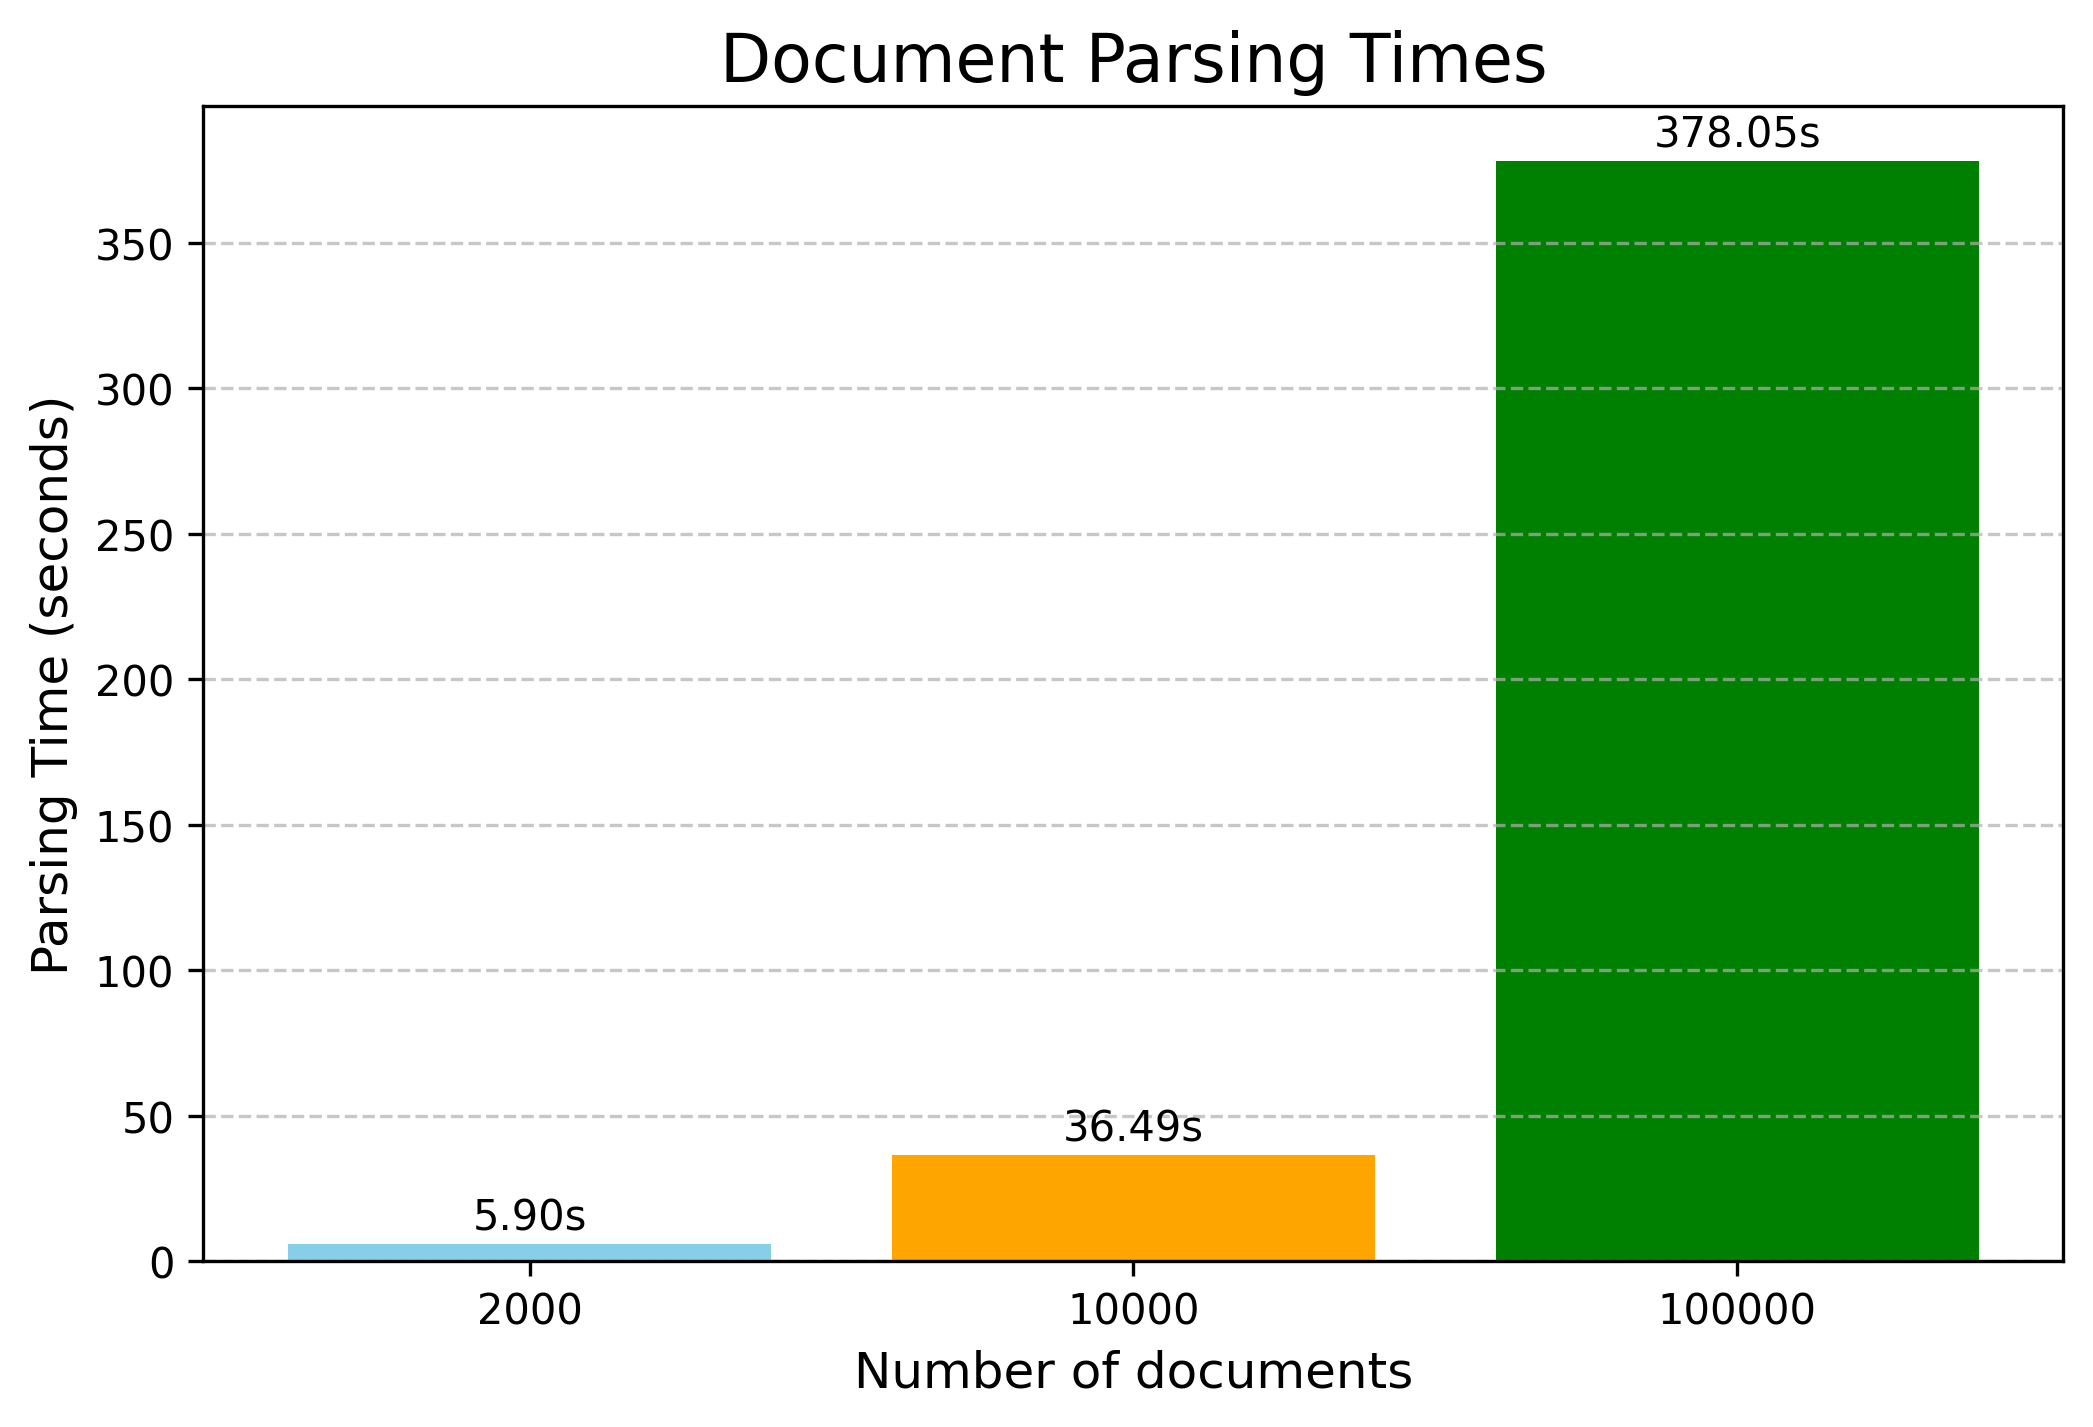
\includegraphics[width=\textwidth]{parsing_times_chart.png}
    \caption{command:'parse'}
    \label{fig:cmd-parse}
\end{figure}
\begin{figure}[h!]
    \centering
    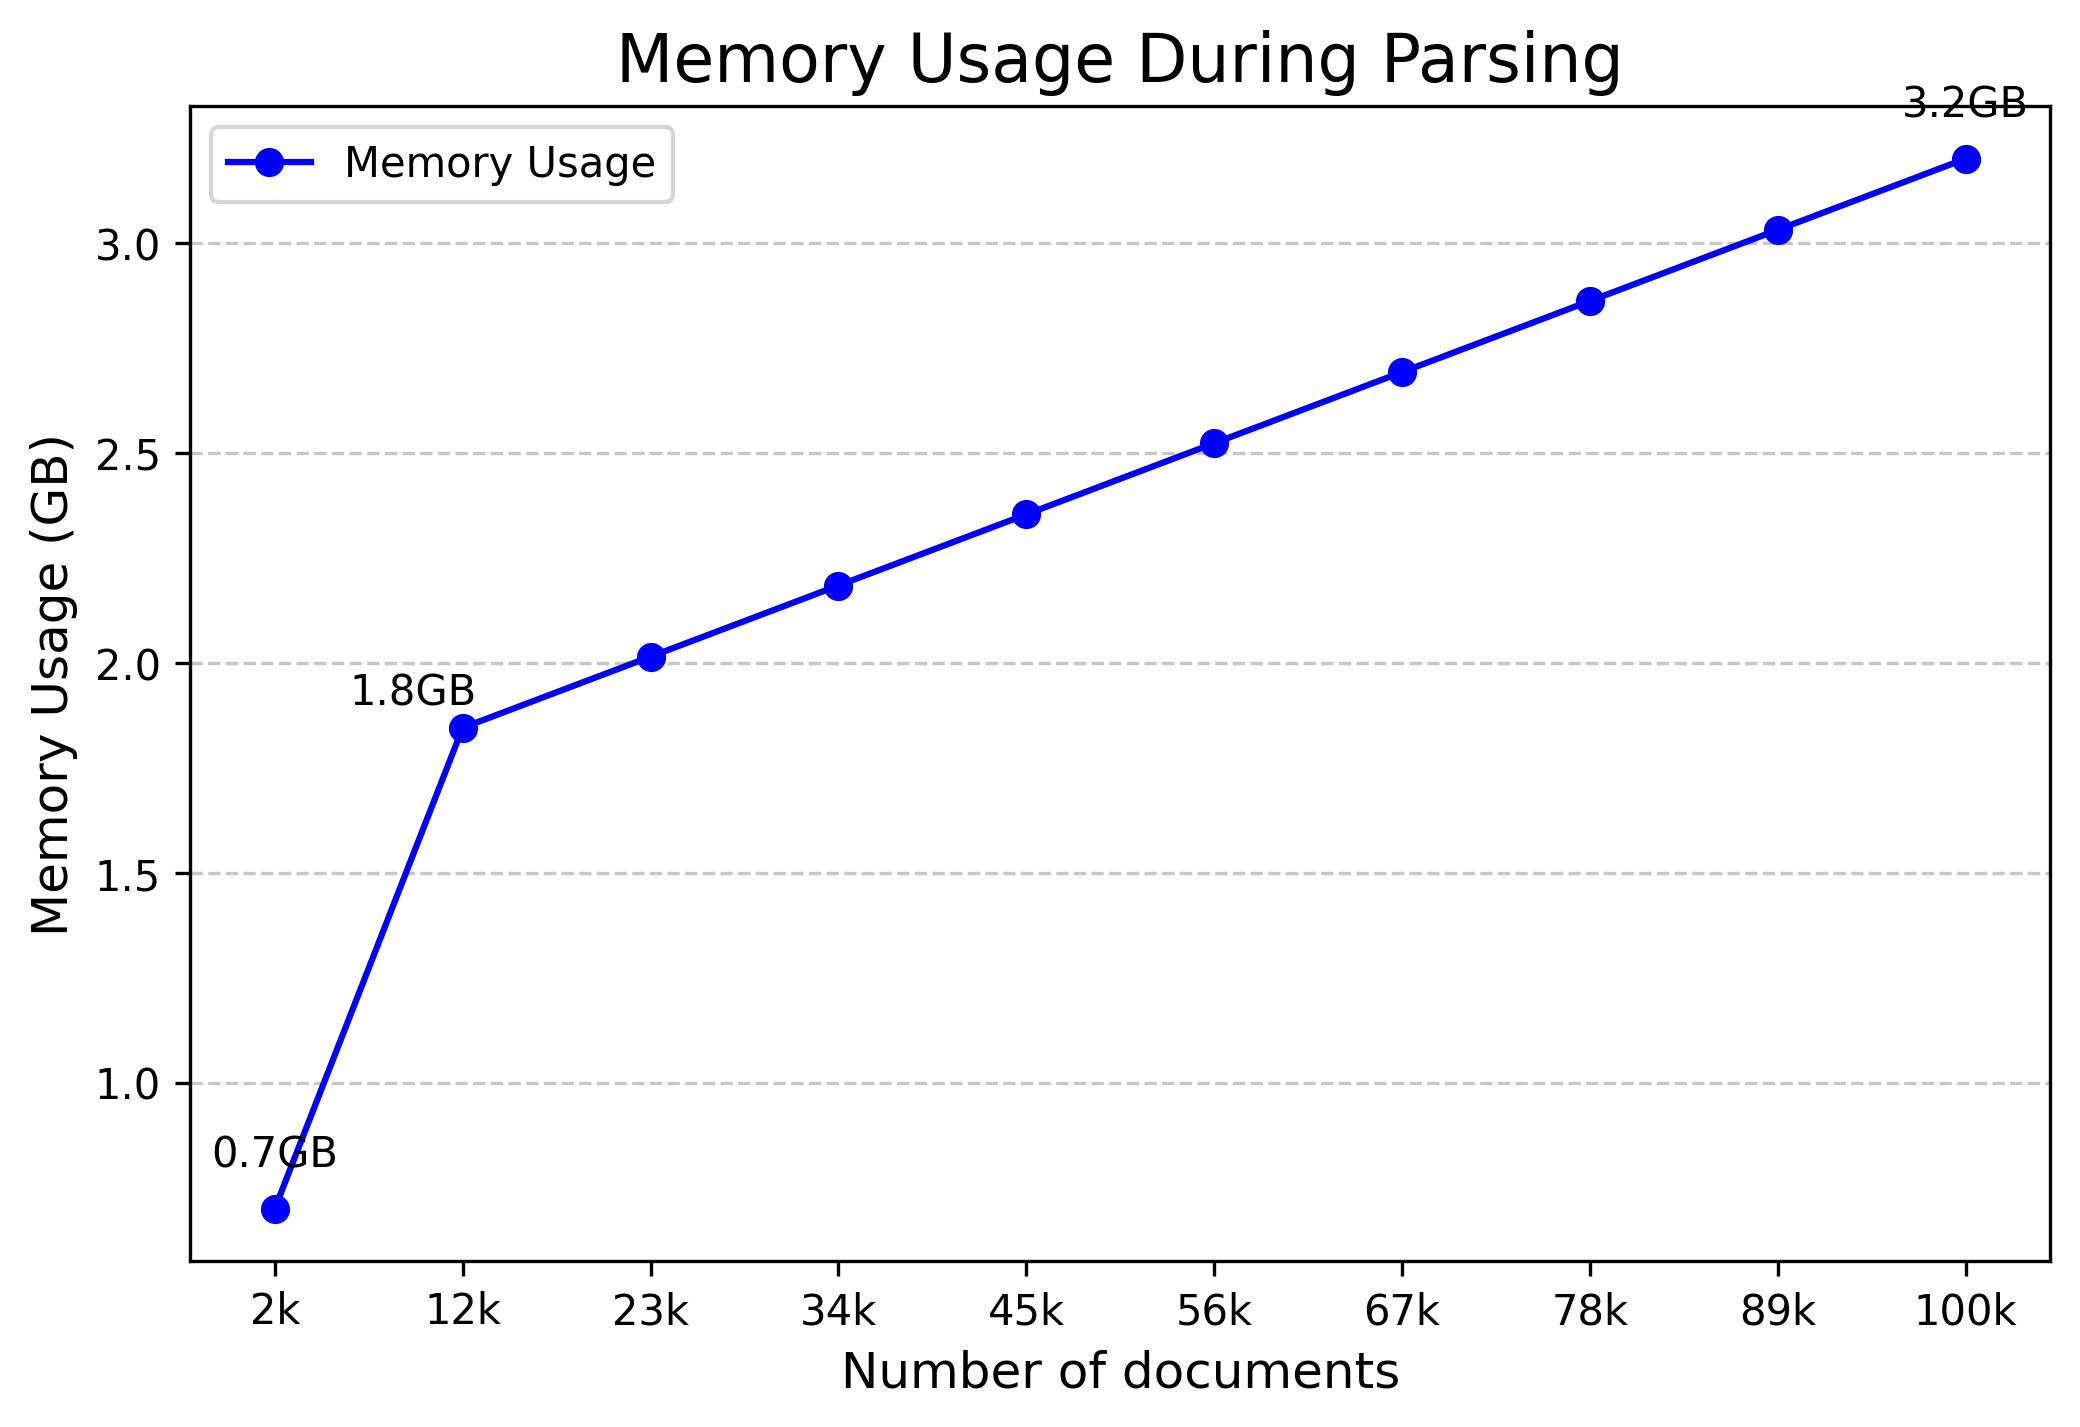
\includegraphics[width=\textwidth]{memory-usage.png}
    \caption{memory usage}
    \label{fig:memory-usage}
\end{figure}

\subsection{Searching}
    \subsection{Initialization}
    To initialize the search engine GoSeek takes less than a second for documents up to 30000 and takes 3 seconds to initialize for 100000 documents. While idle GoSeek uses 1.7GB of memory.
    Figures below  shows correlation between search keywords,memory usage, time it took and number of documents the engine was initialized with for Bitonic Sort and QuickSort algorithms

    \begin{figure}[h!]
        \centering
        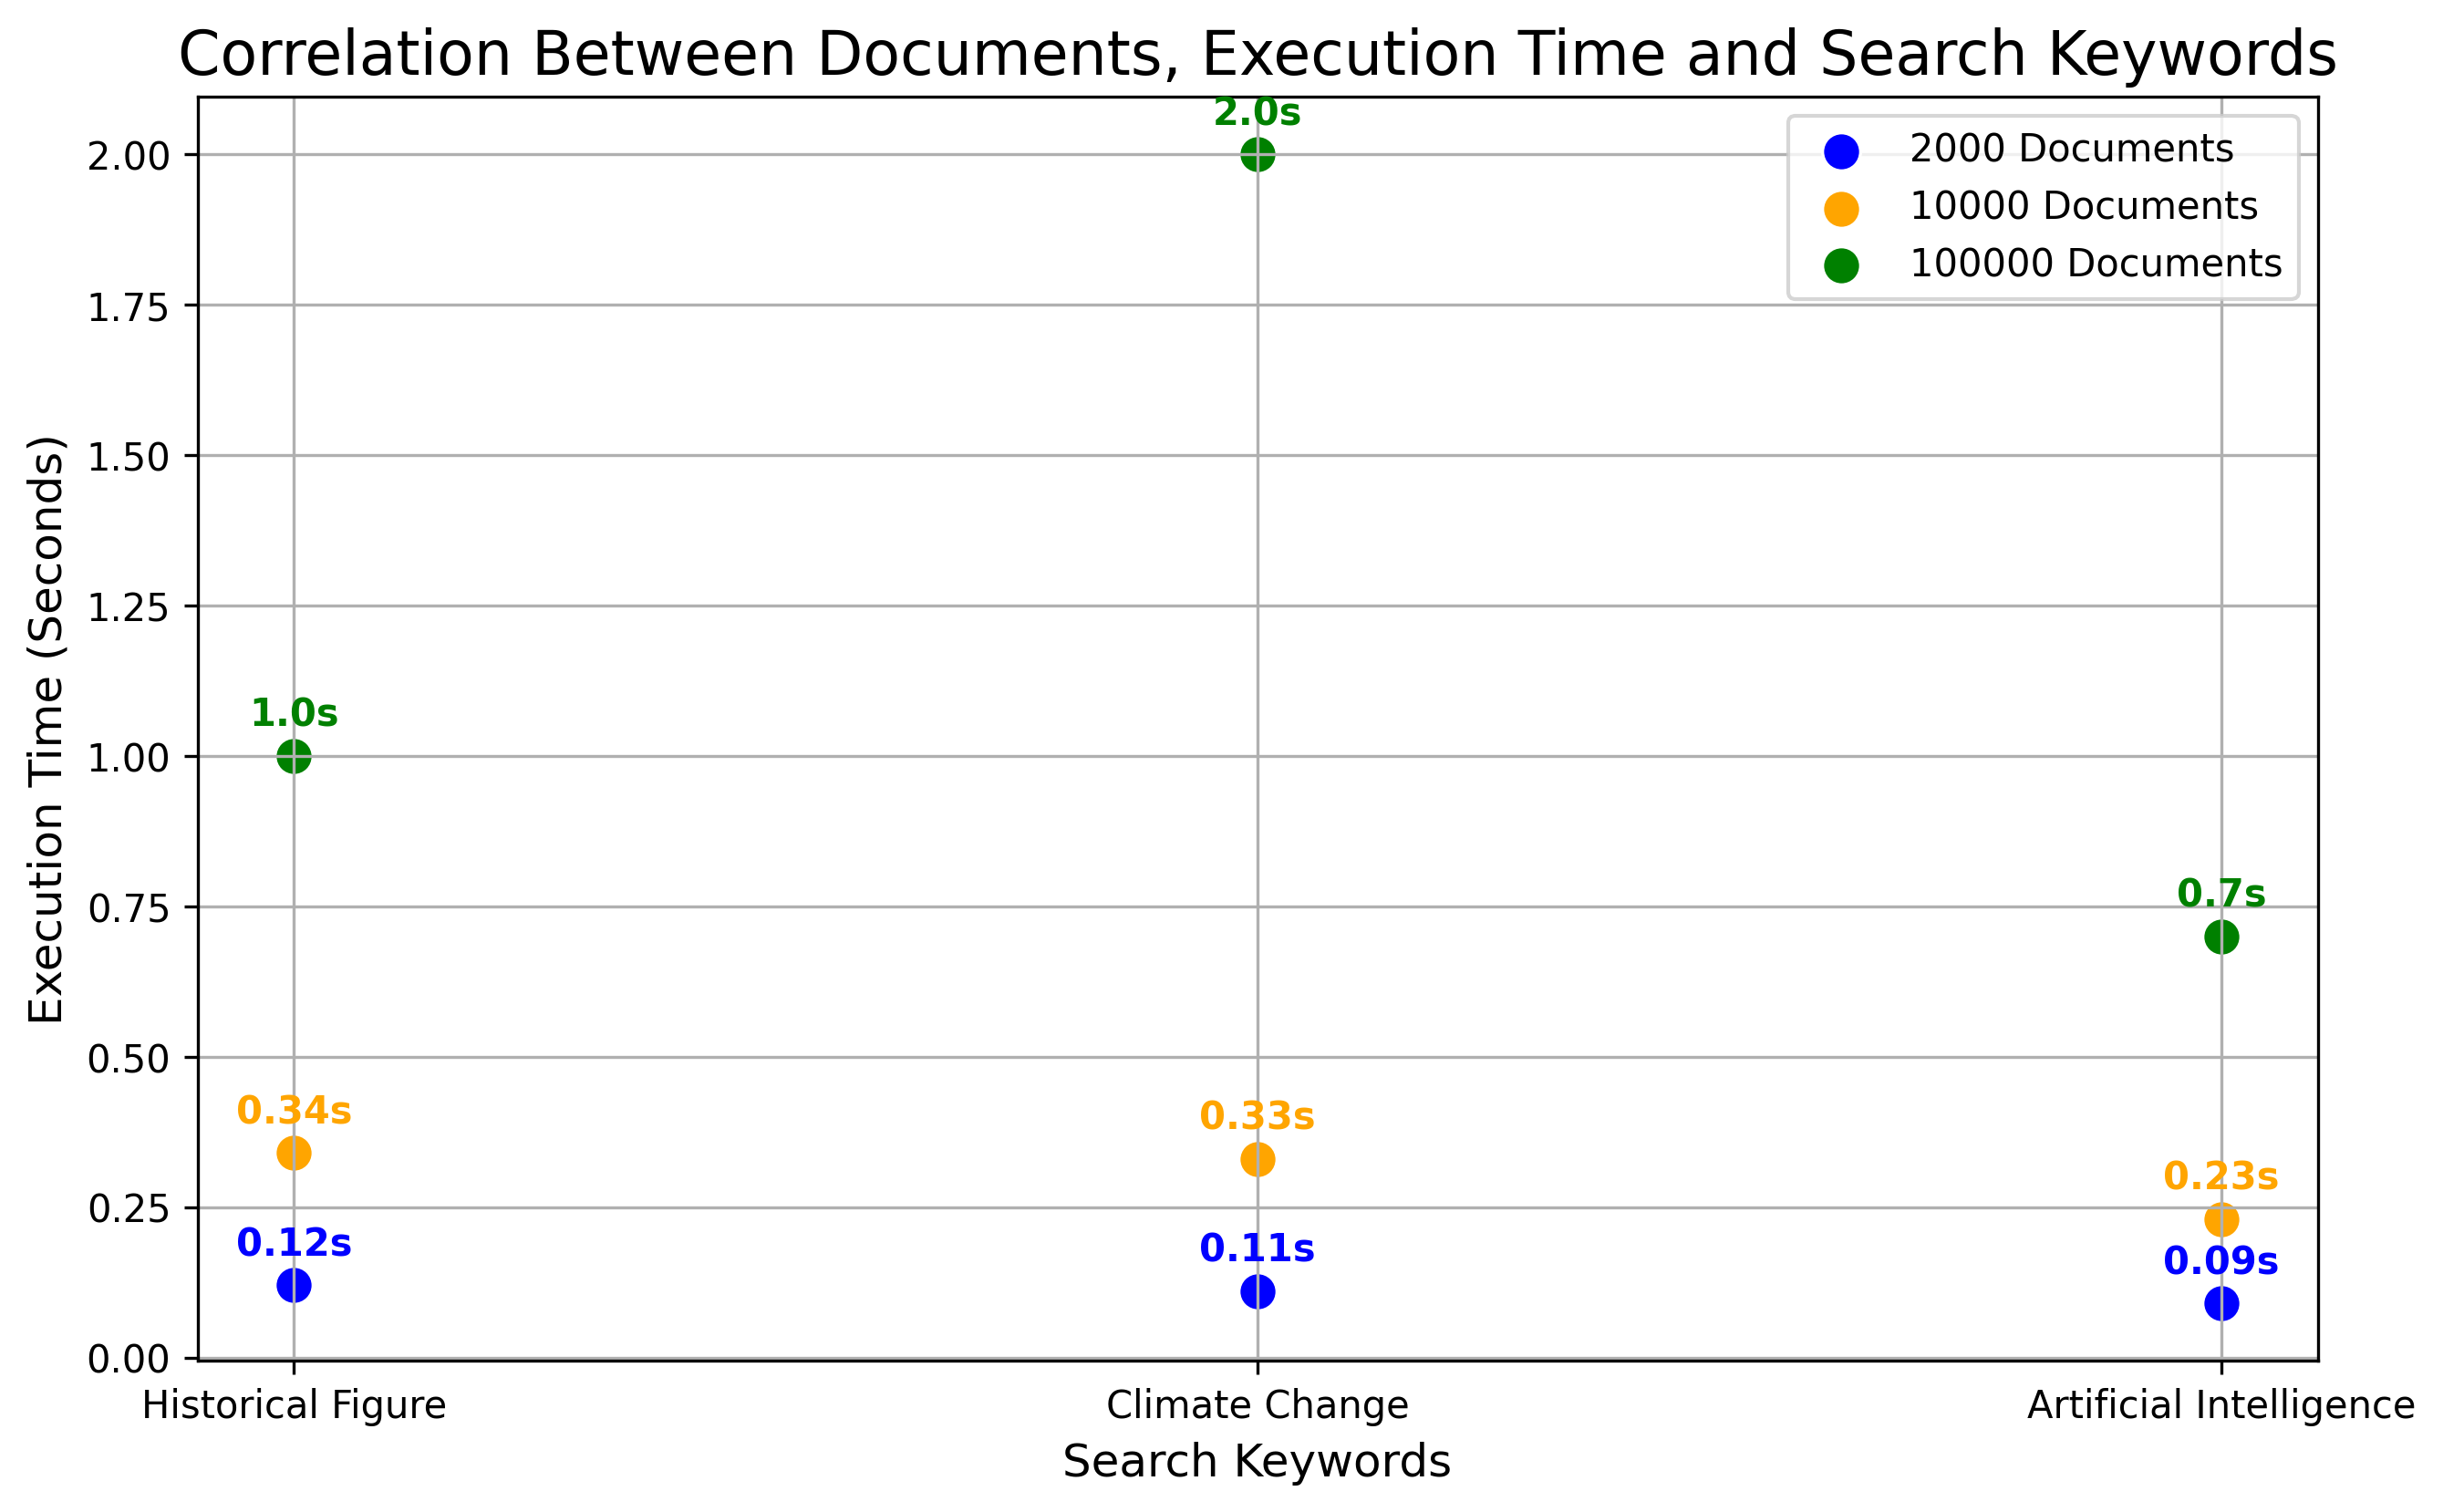
\includegraphics[width=\textwidth]{btsort.png}
        \caption{Bitonic Sort}
        \label{fig:btsort}
    \end{figure}
    \begin{figure}[h!]
        \centering
        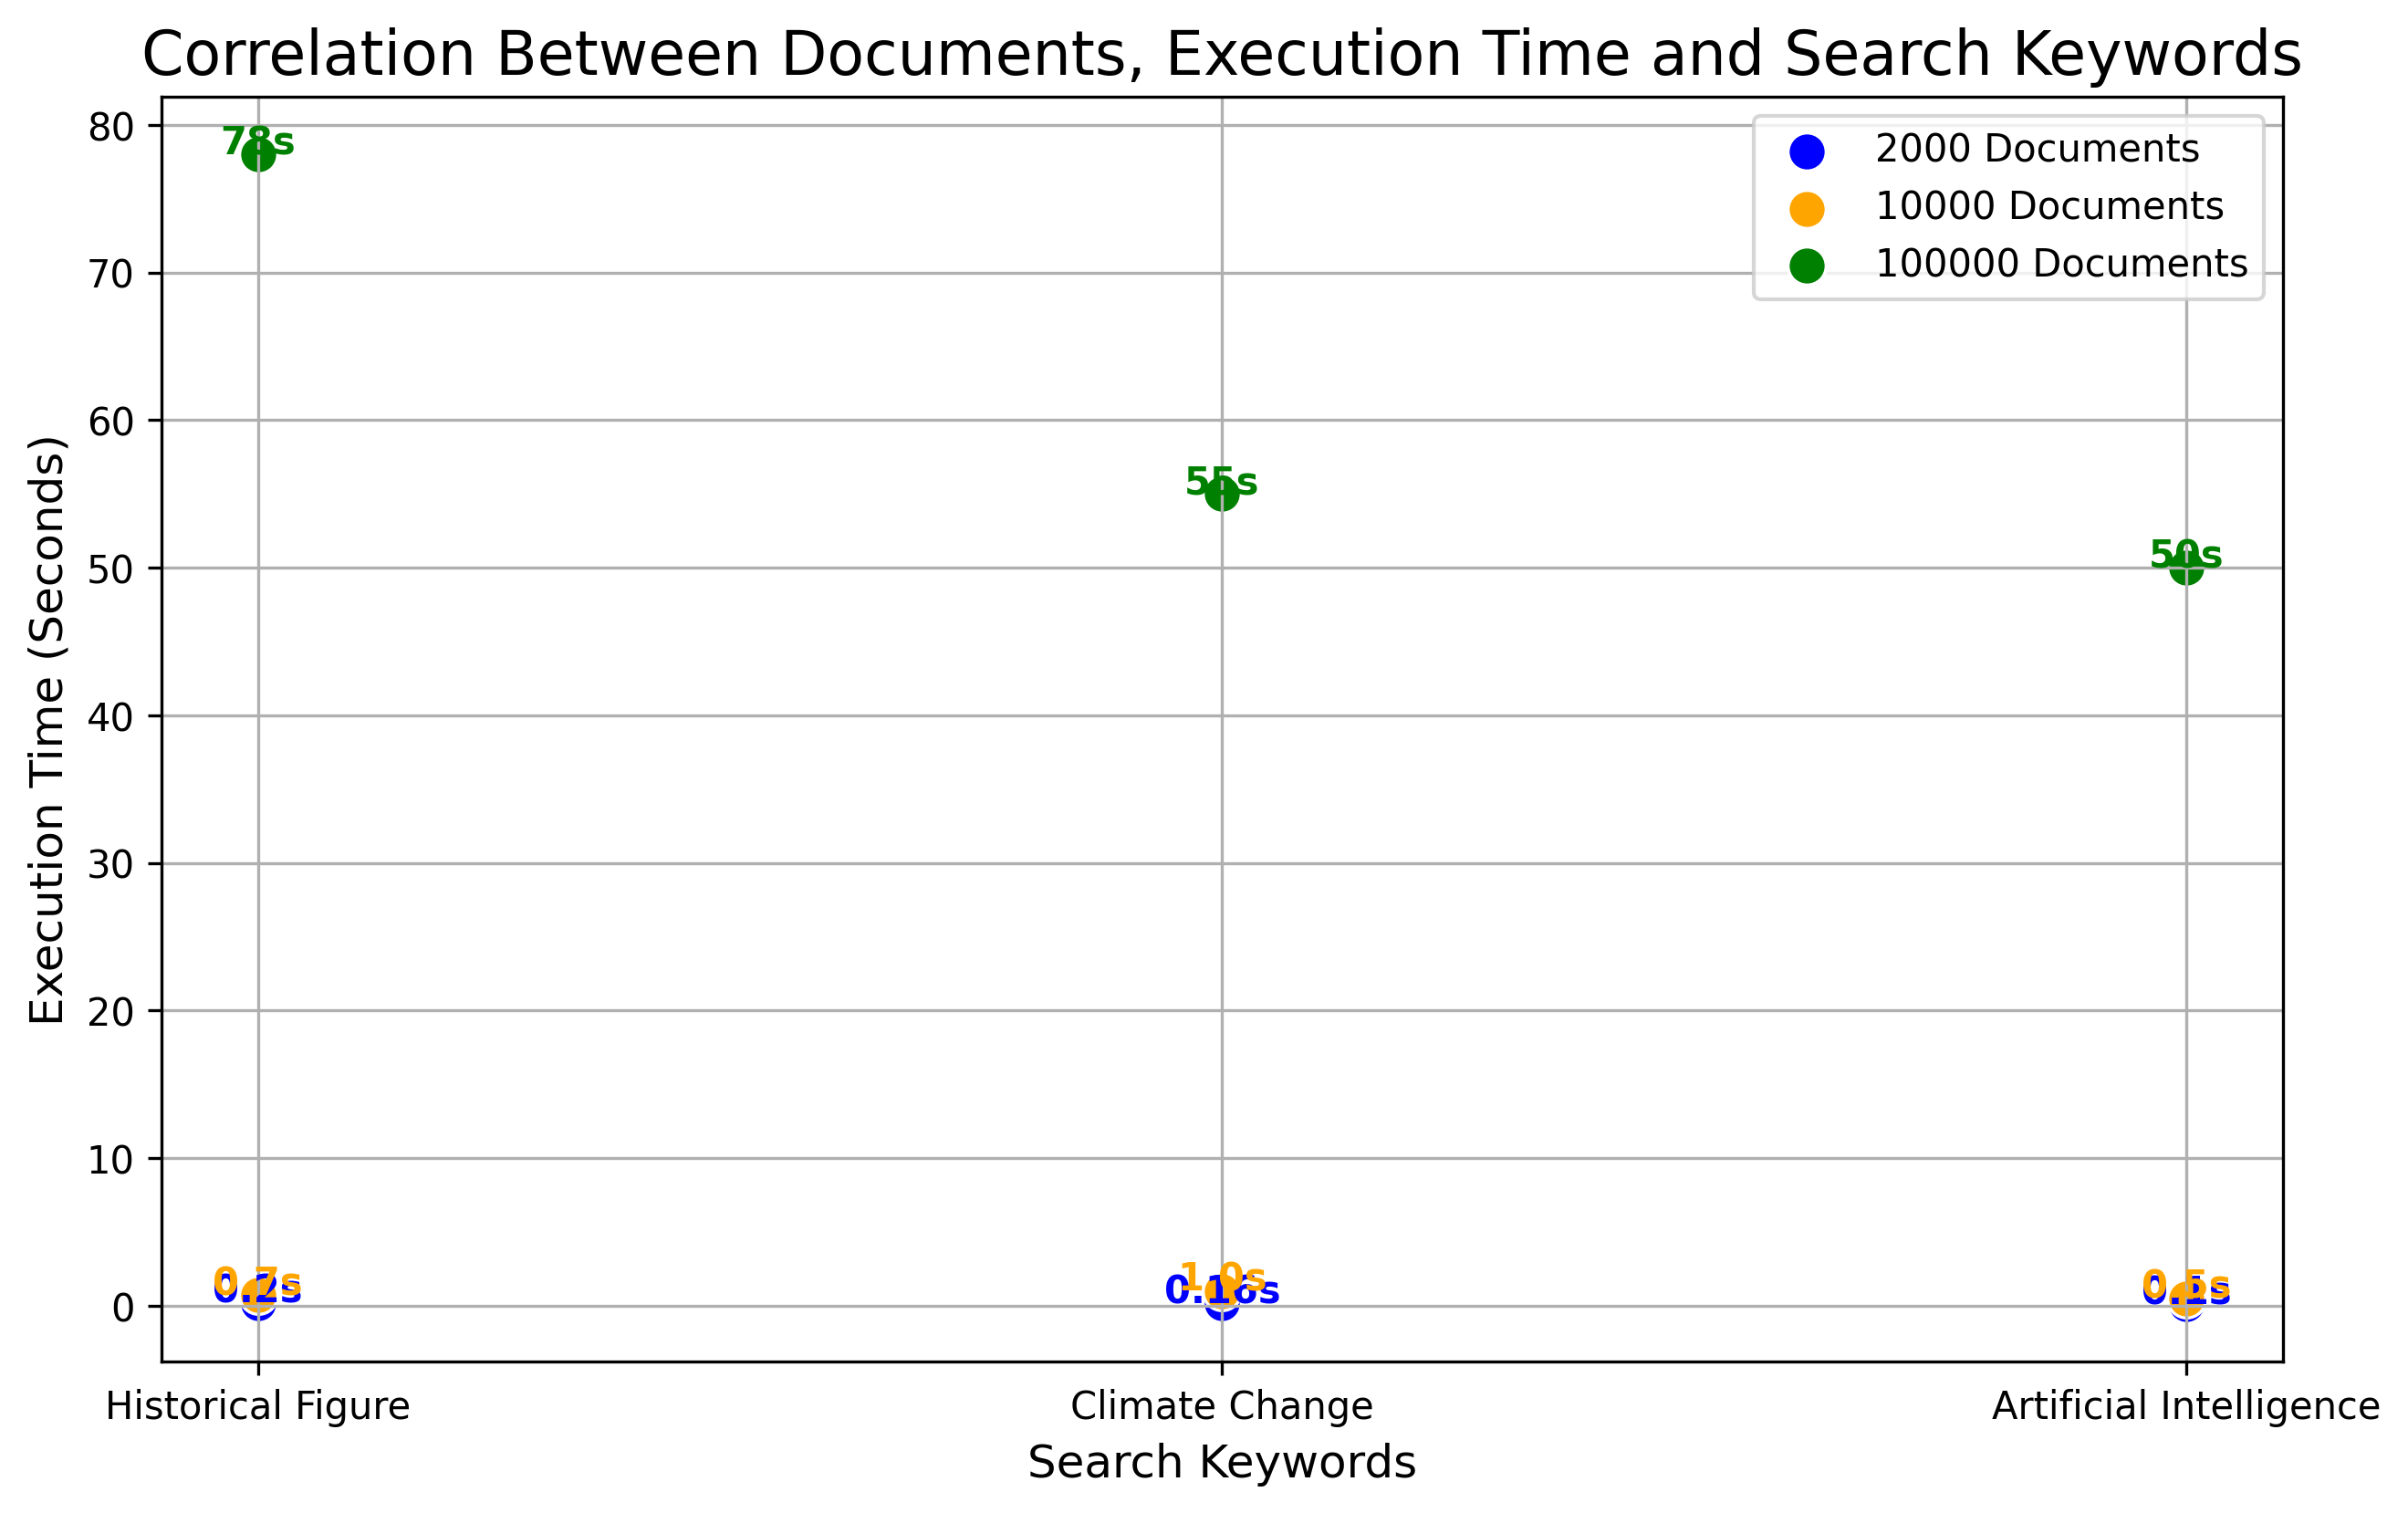
\includegraphics[width=\textwidth]{quicksort.png}
        \caption{Quick-Sort}
        \label{fig:btsort}
    \end{figure}
    \begin{figure}[h!]
        \centering
        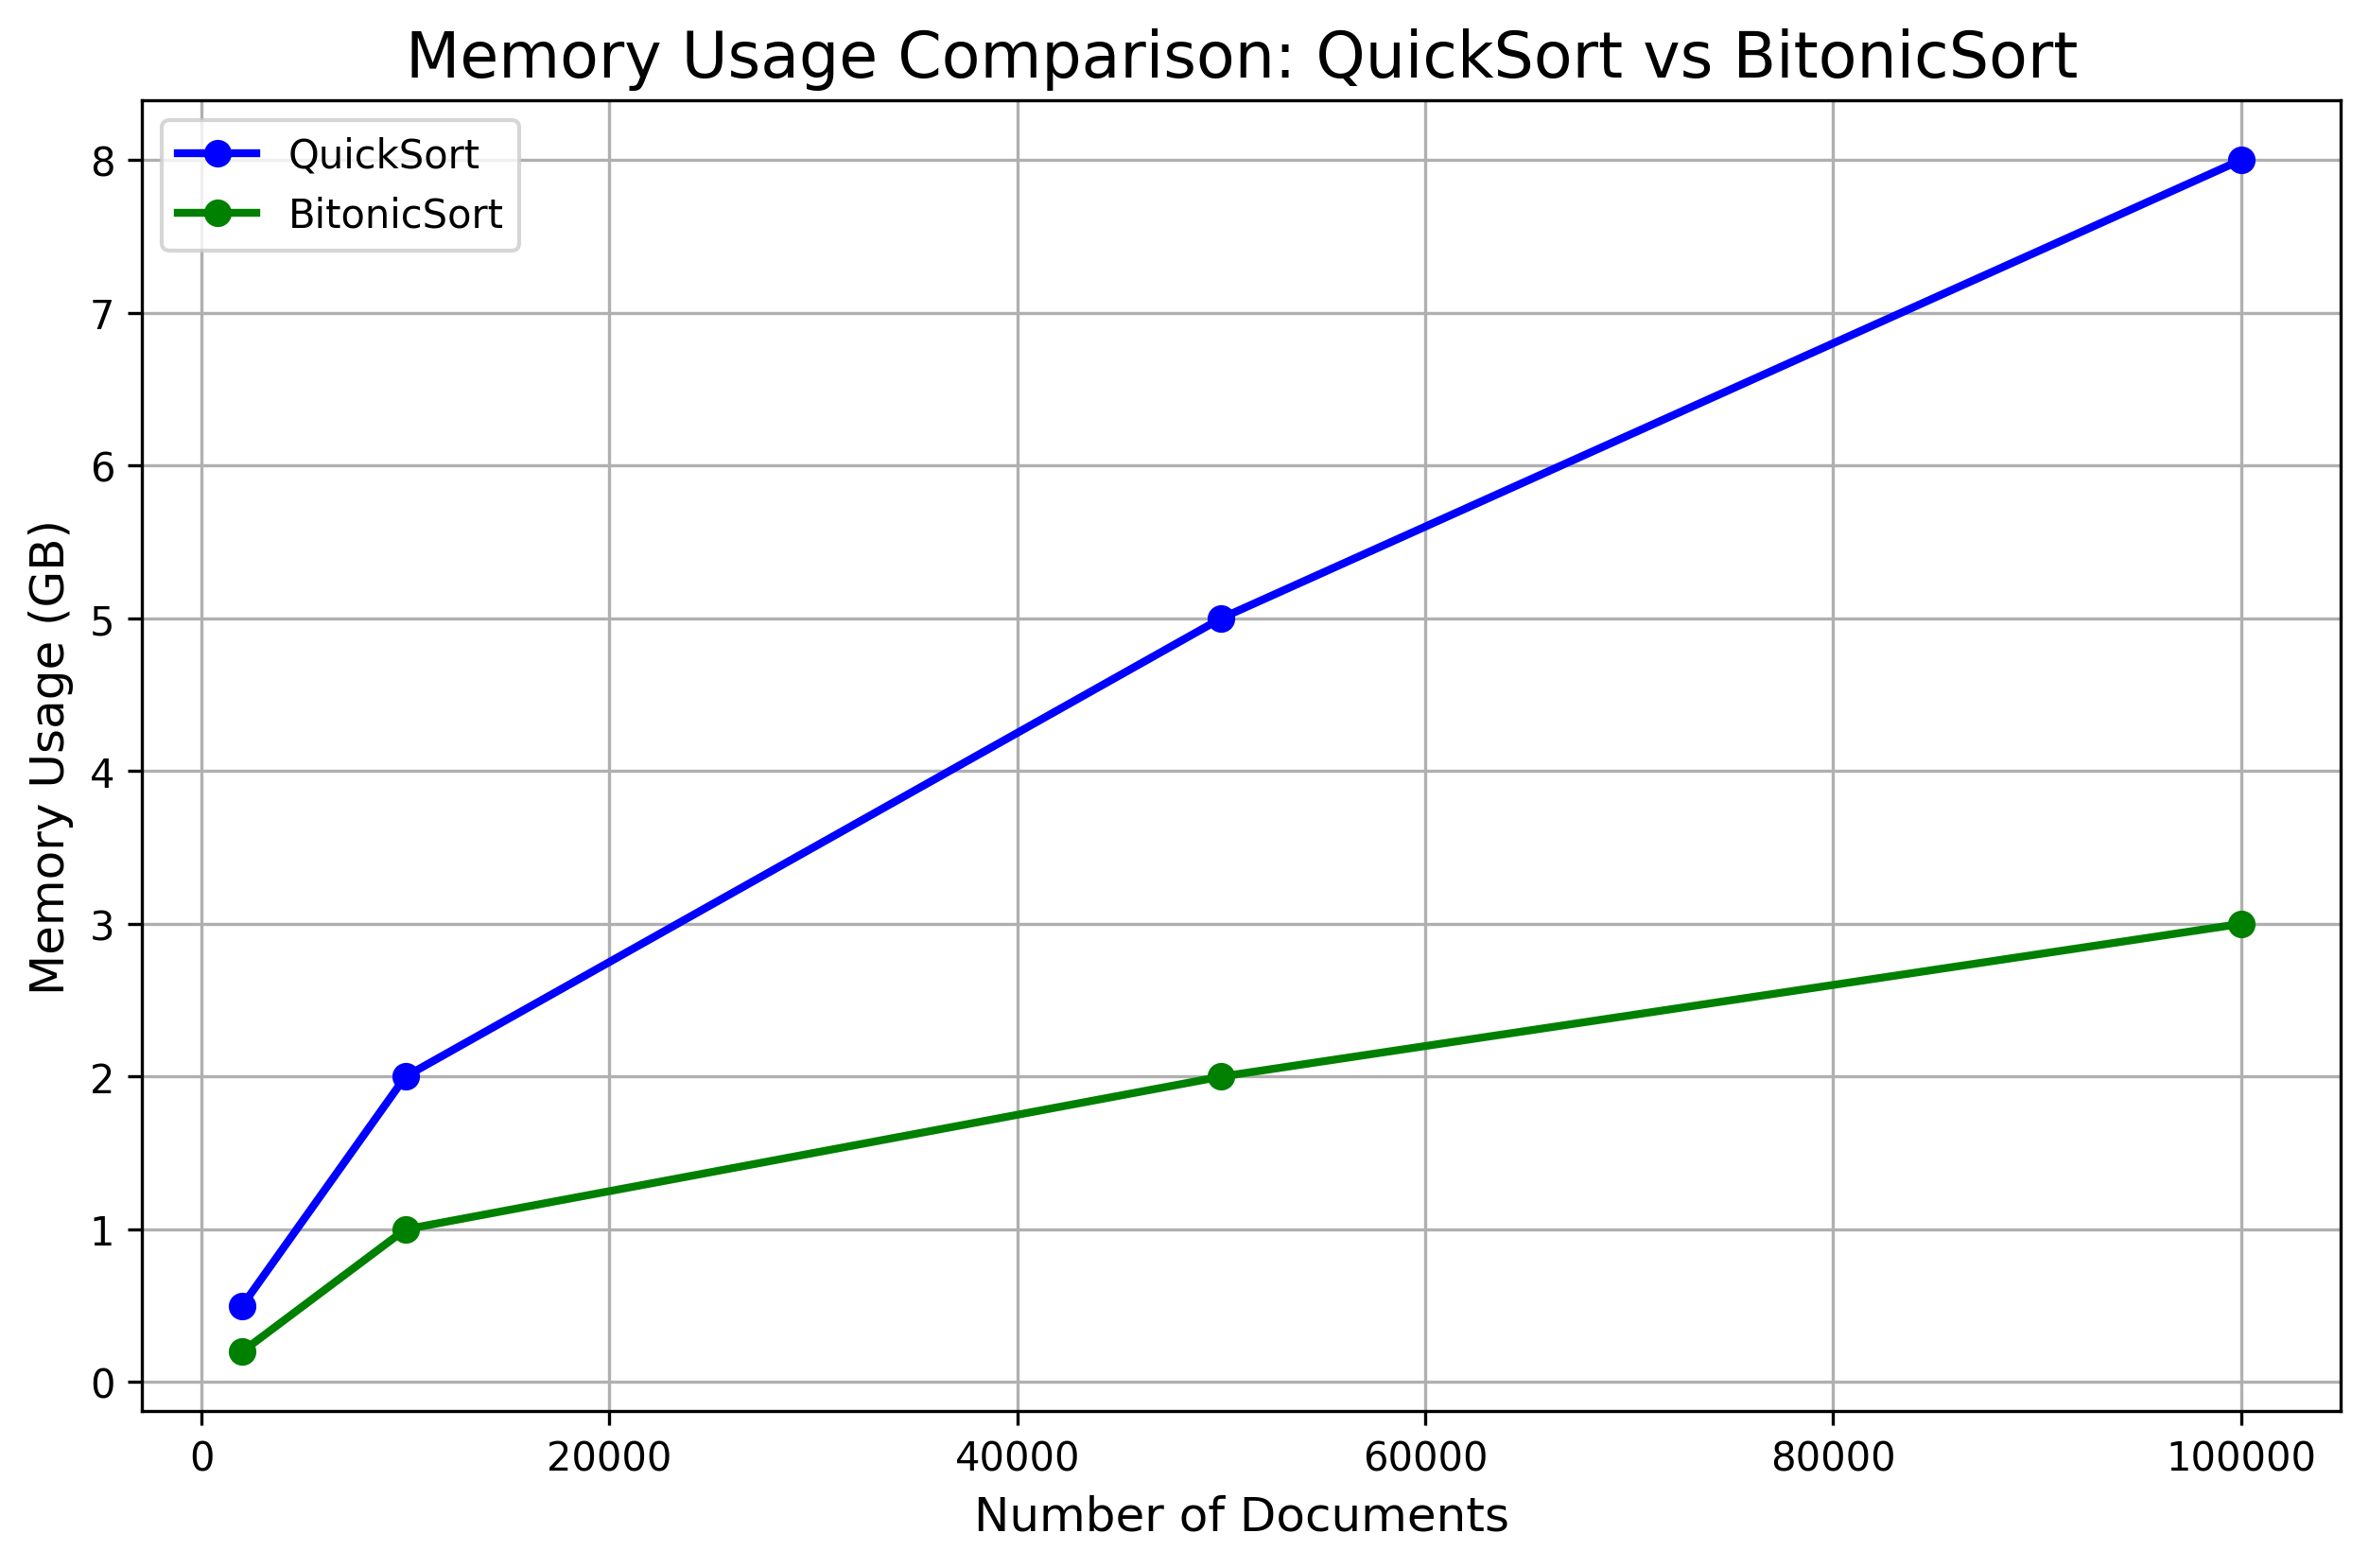
\includegraphics[width=\textwidth]{memory-diff.png}
        \caption{runtime memory usage}
        \label{fig:btsort}
    \end{figure}
    \clearpage
    \subsection{Pattern Matching}
    Pattern matching engine takes less than one second to initialize on all number of documents tested. 
    Figure \ref{fig:pm} below show the correlation between the patterns searched, documents loaded in the engine, and execution time. \\ 
    For more clear understanding of patternMatch capabilities along with the existing \textbf{.json} file , it was tested with 10GB \textbf{.pdf} file. 
    As for memory usage it stays under 800mb.
    \begin{figure}[h!]
        \centering
        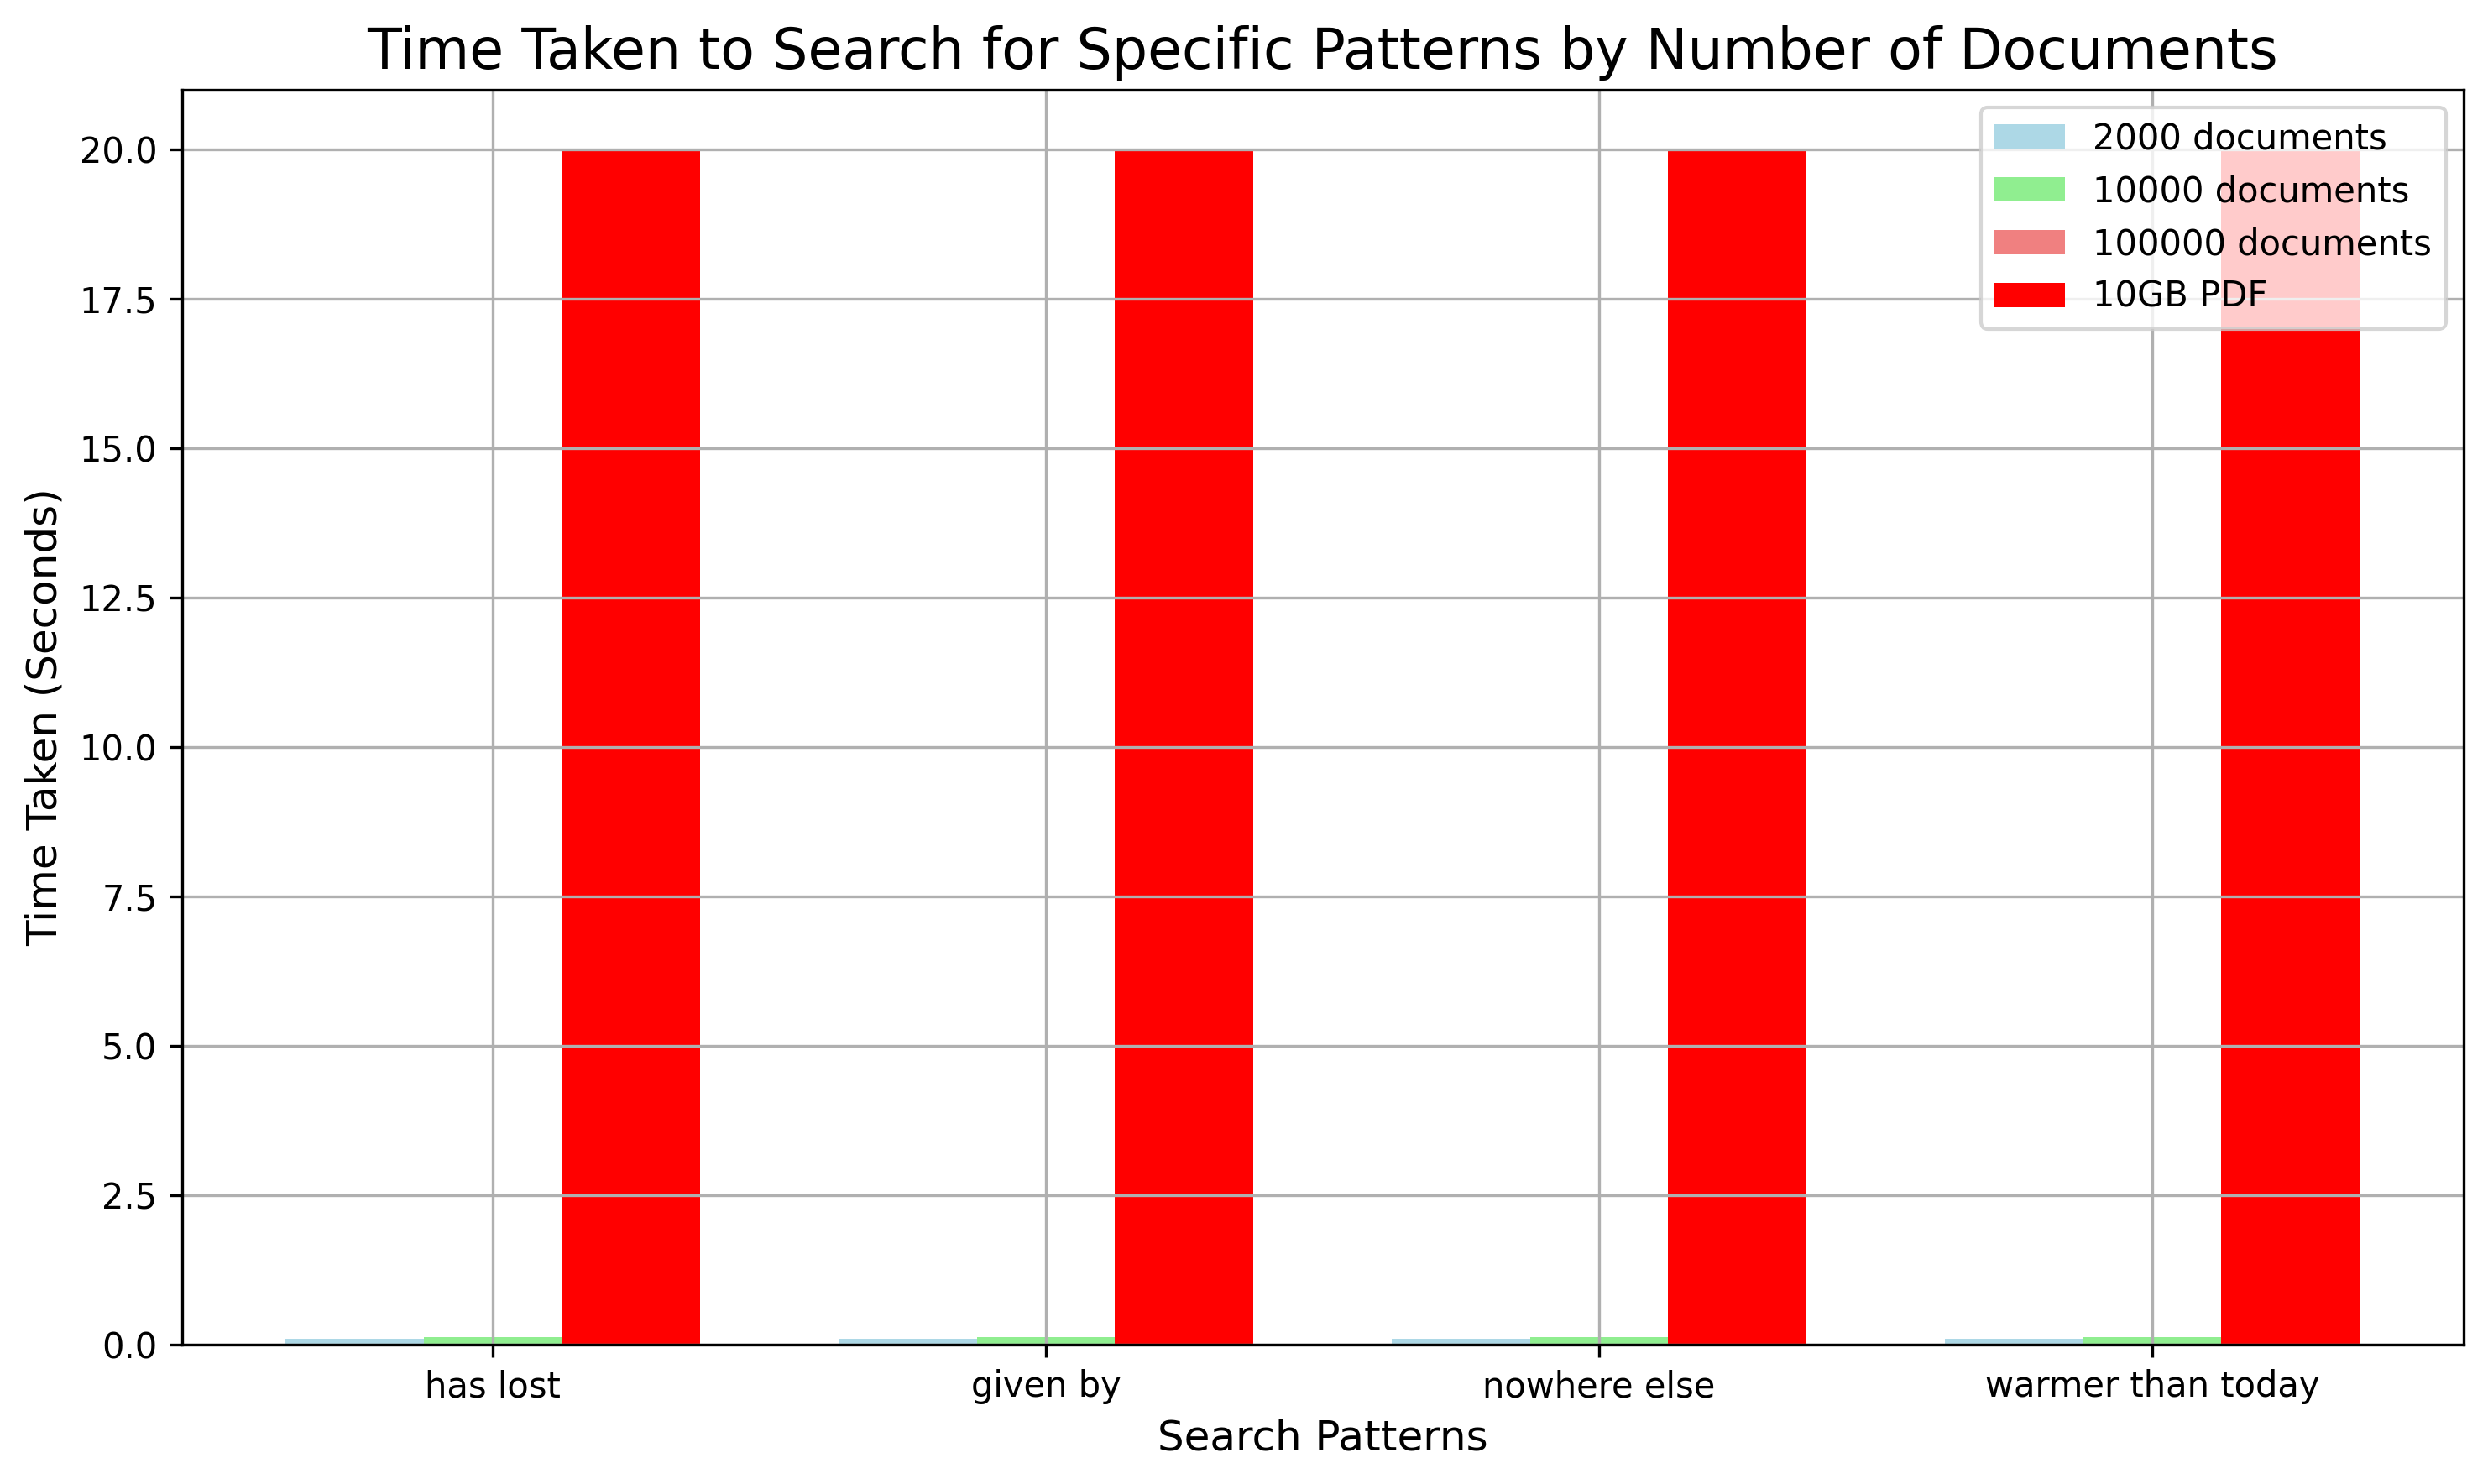
\includegraphics[width=\textwidth]{big-pdf.png}
        \caption{Pattern matching correlations - 300MB input file}
        \label{fig:pm}
    \end{figure}
    \clearpage
\section{Discussion}

The Goseek search engine exhibits outstanding performance and high accuracy when searching for a topic across documents. Its lightweight nature makes it ideal for everyday use by individual users. The tests conducted clearly highlighted the superior performance of the bitonic sort algorithm over other sorting algorithms. Bitonic sort outperformed quicksort by a factor of 76 in terms of speed, while also using significantly less memory. In contrast, quicksort's memory usage increases exponentially as the dataset grows, making it less suitable for large datasets. Additionally, our logs show that bitonic sort does not place a heavy load on CPU usage, operating with fewer than 9,000 concurrent threads, which is easily manageable by modern CPUs. Based on these results, it is safe to conclude that quicksort is not suitable for large datasets. On the other hand, bitonic sort is a scalable and robust solution, even when distributed across multiple machines with the same dataset.

While quicksort is easier to implement and more widely used, it offers no distinct advantages for handling large-scale data. It consumes more memory and is slower in comparison.

The pattern matching engine also demonstrated excellent performance. Searching for a pattern containing three or more words took less than a second in a dataset of 50,000 documents and just 1.2 seconds for 100,000 documents. This demonstrates the efficiency of the Knuth-Morris-Pratt (KMP) algorithm, which processes each character only once. As such, the number of words in the pattern does not significantly impact the execution time. Given this, we can confidently conclude that the KMP algorithm is the ideal choice for all pattern matching applications.

\subsection{Hypothesis Evaluation}

Although we do not have specific comparative data against commercial search engines such as Google or Bing, the results from our implementation show promising potential. Some key highlights include:

\begin{itemize}
    \item Unbiased ranking achieved through the use of Term Frequency-Inverse Document Frequency (TF-IDF)
    \item Advanced pattern matching capabilities
    \item Efficient performance at scale
    \item No advertisement influence on search results
\end{itemize}

\subsection{Strengths}

The Goseek engine possesses several strengths:

\begin{itemize}
    \item Clean, modular architecture adhering to best practices
    \item Comprehensive logging system for performance tracking
    \item Multiple sorting algorithm implementations allowing for performance comparison
    \item Efficient document processing and initialization
    \item Novel combination of TF-IDF with pattern matching
\end{itemize}

\subsection{Weaknesses}

However, there are a few weaknesses:

\begin{itemize}
    \item Limited to a command-line interface
    \item Requires pre-processing of documents before they can be searched
    \item Memory usage could be optimized (1.7GB baseline is significant)
    \item Bitonic sort requires input sizes that are powers of two
\end{itemize}

\subsection{Limitations}

The current work has several limitations:

\begin{itemize}
    \item Testing was conducted on modest hardware (AMD Ryzen 7 3750H, 8GB RAM)
    \item The dataset size used in testing was limited to 100,000 documents
    \item No direct comparison with commercial search engines
    \item The search capability is limited to text in ASCII characters after parsing
\end{itemize}

\subsection{Future Work}
Future work will involve the development of a web interface to make the engine more accessible. By adding a user-friendly interface, Goseek can reach a wider audience, moving beyond its current command-line configuration. \\
Currently GoSeek is great at describing internal processes but analyzing them is up to the user, thus one great addition would be a analyzer command that tells the user \\
all of the performance evaluations based on the already existing logs in a manner which is more readable and accessible to the user.
